\subsection{Medición de la resistencia interna de un amperímetro} \label{sec:resistencia de amp}
\paragraph{}
En esta sección, se midió la resistencia interna de un amperímetro. Para esto, se armó el circuito de la figura \ref{fig:esq_amperimetro} usando una fuente de diferencia de potencial constante, una resistencia variable, un amperímetro y un voltímetro. 

\begin{figure}[H]
    \centering
    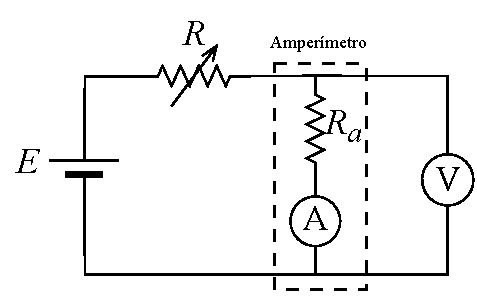
\includegraphics[width = 0.5\linewidth]{Esquemas/Resistencia amperimetro.pdf}
    \caption{Esquema que representa a un circuito eléctrico dotado de una fuente de voltaje constante $E$, una resistencia variable $R$, un amperímetro modelado como una resistencia interna $R_a$, un amperímetro ideal (de resistencia cero), y un voltímetro. Al conectar el voltímetro en paralelo, su resistencia interna (calculada en la sección \ref{sec:resistencia de volt}) es despreciable. Se utilizaron valores de $R$ tal que $R \gg R_a$}
    \label{fig:esq_amperimetro}
\end{figure}
\paragraph{}
En este circuito, y al igual que en la sección \ref{sec:resistencia de volt}, la resistencia variable $R$ se modifica para obtener distintos valores de caída de potencial y corriente, con el fin de determinar $R_a$. Se registraron los valores de corriente dados por el amperímetro, y la caída de potencial en el mismo con el voltímetro. Se realizó un ajuste utilizando la ley de Ohm (Ec. \ref{eqn:ley de ohm}) con $R_a$ y los datos obtenidos.

\begin{figure}[H]
    \centering
    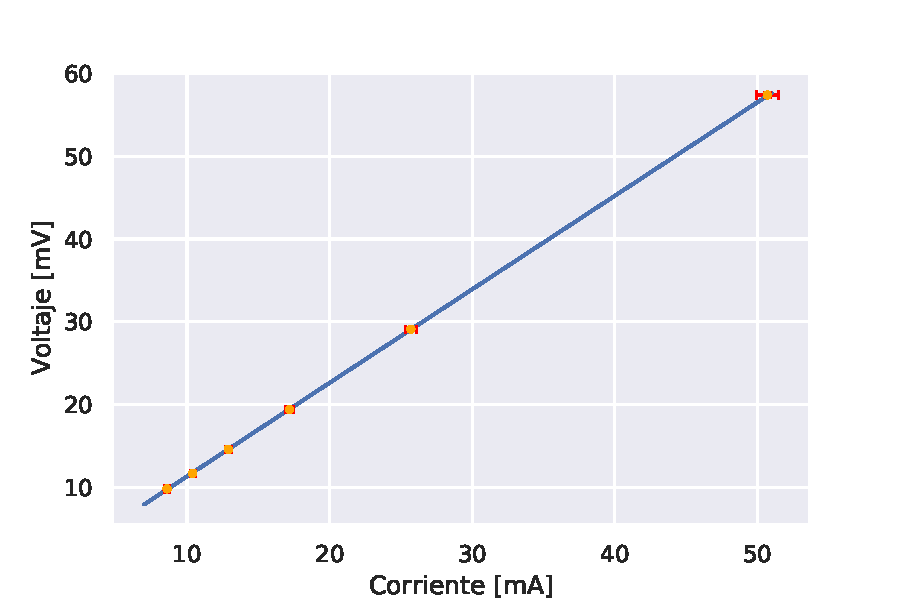
\includegraphics[width = 0.65\linewidth]{figuras/amperimetro.pdf}
    \caption{Ajuste lineal de las mediciones de voltaje en función de la corriente. Como puede observarse, el voltaje aumenta proporcionalmente con la corriente a medida que se modifica el valor de $R$.}
    \label{fig:fig_amperimetro}
\end{figure}

\paragraph{}
Se obtuvo un valor de la resistencia de $R_a=(1.13 \pm 0.01)$ $\Omega$. Este valor es razonable, ya que una resistencia pequeña permite que circule la mayor cantidad de corriente posible a través del instrumento. En este caso, una resistencia de alrededor de 1 $\Omega$ es adecuada para medir la corriente en un circuito en el que las resistencias se encuentran en el orden de $10^{3}$ $\Omega$.